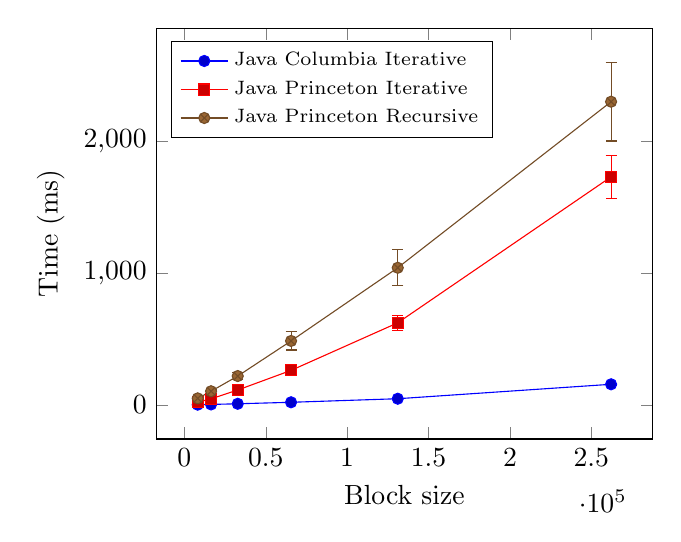
\begin{tikzpicture}
\begin{axis}[xlabel={Block size},ylabel={Time (ms)},width=0.65\linewidth,legend pos=north west,scaled y ticks = false,legend cell align=left,legend style={font=\scriptsize}]
\addplot+[error bars/.cd, y dir=both,y explicit] coordinates {
(8192, 2.1766) +- (0.3256, 0.3256)
(16384, 3.9995) +- (0.4596, 0.4596)
(32768, 8.9846) +- (1.3089, 1.3089)
(65536, 20.2833) +- (2.4423, 2.4423)
(131072, 47.2950) +- (6.6700, 6.6700)
(262144, 156.7135) +- (6.0892, 6.0892)
};
\addplot+[error bars/.cd, y dir=both,y explicit] coordinates {
(8192, 21.1757) +- (4.9079, 4.9079)
(16384, 46.8150) +- (9.6619, 9.6619)
(32768, 113.1953) +- (11.0218, 11.0218)
(65536, 261.9954) +- (13.8293, 13.8293)
(131072, 622.4328) +- (57.9001, 57.9001)
(262144, 1728.4640) +- (161.0712, 161.0712)
};
\addplot+[error bars/.cd, y dir=both,y explicit] coordinates {
(8192, 50.0776) +- (7.5896, 7.5896)
(16384, 103.9682) +- (15.7929, 15.7929)
(32768, 219.0208) +- (28.3890, 28.3890)
(65536, 485.1020) +- (68.2330, 68.2330)
(131072, 1039.4937) +- (137.6356, 137.6356)
(262144, 2297.8011) +- (297.4241, 297.4241)
};
\legend{Java Columbia Iterative , Java Princeton Iterative , Java Princeton Recursive}
\end{axis}
\end{tikzpicture}
